\chapter{Problemanalyse} \label{cha:problemanalyse}

\section{Anforderungen und Problemabgrenzung} \label{cha:problemanalyse:abgrenzung}

Die Schnitzeljagden sollen in erster Linie den Studienanfängern (Ersties) dienen, um ihnen auf interaktive Weise den Campus nahe zu bringen und sie mit den wichtigsten Orten und Einrichtungen vertraut zu machen.

Im Rahmen des Projekts wurden folgende Ziele in einer Vier-Felder-Matrix aufgeteilt.

\begin{figure}[H]
    \centering
    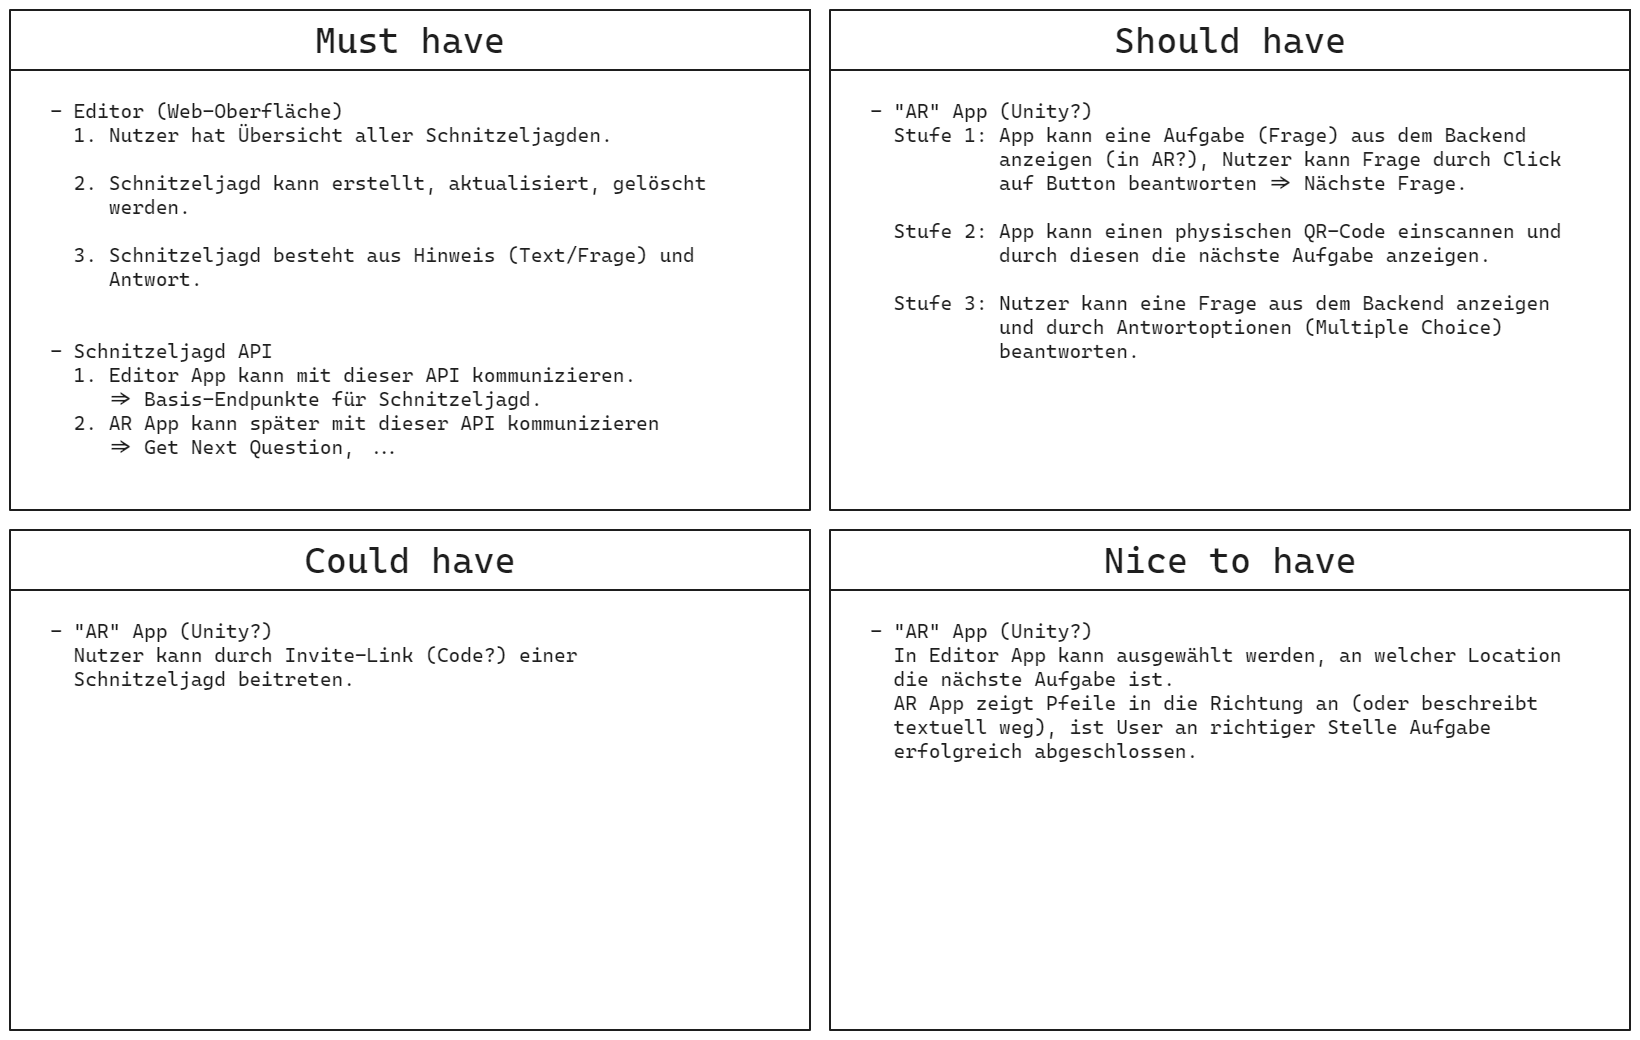
\includegraphics[width=\textwidth]{images/PrAr_ProblemAnalysis_Vierfelder.png}
    \caption{Darstellung der Projekt-Ziele aufgeteilt in Vier Felder}
    \label{fig:problemanalyse:vierfeldermatrixamarsch}
\end{figure}

Für die erfolgreiche Projektumsetzung sind folgende Eigenschaften zu berücksichtigen.

\subsubsection{Flexibilität}

Ein wichtiger Aspekt des Projekts ist, dass eine Schnitzeljagd so flexibel wie möglich durchgeführt werden soll. Eine Aufgabenstellung und die dazu gehörende Lösung sollten hierbei entkoppelt und dynamisch erweiterbar sein, ohne einen größeren Aufwand in der Implementierung zu benötigen.

\subsubsection{Skalierbarkeit}

Das System muss in der Lage sein, mehrere Schnitzeljagden gleichzeitig durchzuführen, ohne dass es zu Problemen kommt. Es sollte möglich sein, die Ressourcen des Systems dynamisch entsprechend der Anzahl der aktuell aktiven Benutzer zu skalieren, ohne dass dabei Performanceeinbußen oder ähnliche Beeinträchtigungen auftreten.

\subsubsection{Benutzerfreundlichkeit}

Der Anmelde- und Durchführungsprozess sollte unabhängig voneinander klar strukturiert sein, um den Benutzern eine reibungslose und intuitive Erfahrung zu bieten. Während der Durchführung der Schnitzeljagd sollten keine Schwierigkeiten auftreten. Die Schnitzeljagd soll den Benutzern eine einzigartige Erfahrung bieten, ohne durch unnötige oder ablenkende Elemente zu stören. Idealerweise fungiert die Anwendung als Schnittstelle zur Durchführung der Schnitzeljagd, wobei das Lösen der Aufgaben direkte Interaktionen im realen Leben erfordert.

Die digitale Plattform ermöglicht eine einfache Anmeldung und Durchführung der Schnitzeljagd, wodurch der organisatorische Aufwand minimiert und die Zugänglichkeit maximiert wird.

\subsubsection{Sicherheit}

Das Thema Sicherheit ist im Bezug auf sensible Benutzerdaten wie Passwörter sehr wichtig. Durch die architektonischen Überlegungen die in Kapitel \ref{cha:swentwurf} beschrieben werden, wäre es möglich im Anschluss die Benutzerdaten durch kryptographisch sichere Hashfunktionen zu speichern. Um den Projektumfang auf das Wesentliche zu reduzieren, wurde dies im Projekt nicht berücksichtigt.

\section{Architektonische Überlegungen}

Bei der Wahl einer angemessenen Architektur für das System sind viele Aspekte zu berücksichtigen, unter anderem die in Kapitel \ref{cha:problemanalyse:abgrenzung} genannten Eigenschaften.

In Kapitel \ref{cha:swentwurf} wird daher der service-orientierte Ansatz für den Entwurf der Software allumfassend beschrieben.
